% =============================================================================
% supplementary.tex -- Supplementary Information (SI) for the JMD manuscript.
%
% Detailed development records that do not belong in the main manuscript are
% collected here per the PR #20 review (@sgbaird): the main text stays
% high-level and free of GitHub/PR-specific references, while the SI may cite
% specific pull requests and link to them directly.
%
% Build:  cd manuscript && pdflatex supplementary  (twice)
%         or  make manuscript-si
% =============================================================================
\documentclass[11pt]{article}

\usepackage[margin=1in]{geometry}
\usepackage{graphicx}
\usepackage{booktabs}
\usepackage{siunitx}
\usepackage{amsmath}
\usepackage{xcolor}
\usepackage[colorlinks=true,urlcolor=blue,linkcolor=black]{hyperref}

% Synthetic-placeholder (dummy) data convention, matching the main text:
% any stand-in value is typeset in violet. None remain as of 2026-09-15.
\definecolor{dummydata}{RGB}{142,68,173}
\newcommand{\dummy}[1]{\textcolor{dummydata}{#1}}

% Number SI floats/sections with an "S" prefix.
\renewcommand{\thesection}{S\arabic{section}}
\renewcommand{\thefigure}{S\arabic{figure}}
\renewcommand{\thetable}{S\arabic{table}}

\newcommand{\repo}{https://github.com/vertical-cloud-lab/tensegrity-optimization}

\title{Supplementary Information:\\
  Experiment-Driven Bayesian Optimization of the Impact Response of\\
  Multi-Material 3D-Printed Tensegrity-Inspired Structures}
\author{}
\date{}

\begin{document}
\maketitle

\begin{center}
  \fcolorbox{dummydata}{dummydata!6}{\parbox{0.94\linewidth}{\small
  \textcolor{dummydata}{\textbf{Draft note (remove before submission):}
  as in the main text, any value printed in this violet color is a
  synthetic placeholder rather than a measurement. As of 2026-09-15
  this Supplementary Information contains no violet values: the
  former placeholder batch-2 print key was replaced by the logged
  campaign record, which now covers batches 2 to 4.}}}
\end{center}

This Supplementary Information collects the detailed design-, fabrication-,
test-, and analysis-development records supporting the main manuscript. Unlike
the main text, the SI references the project's development history directly,
including specific pull requests (PRs) and issues in the project repository
(\href{\repo}{\repo}).

% -----------------------------------------------------------------------------
\section{Joint-Design Study}
\label{si:joints}
% -----------------------------------------------------------------------------
The strut-to-cable junction was developed and ranked through a five-design
OpenSCAD study (anchor-bulb, dovetail, TPU-sleeve overmold, eyelet-loop, and
TPU-rebar variants). The working prototype uses a dovetail joint (Design~B)
with an anchor-bulb backup (Design~A) for sensitivity studies; a captive TPU
core is routed inside the PLA shell so that the soft tendon is protected from
layer-line failure at the transition.

Full results, renders, and the Phase-3/Phase-4 design reviews are documented in
\href{\repo/pull/39}{PR~\#39} (joint design) and
\href{\repo/pull/35}{PR~\#35} (CAD parameterization and print history).

\begin{figure}[ht]
  \centering
  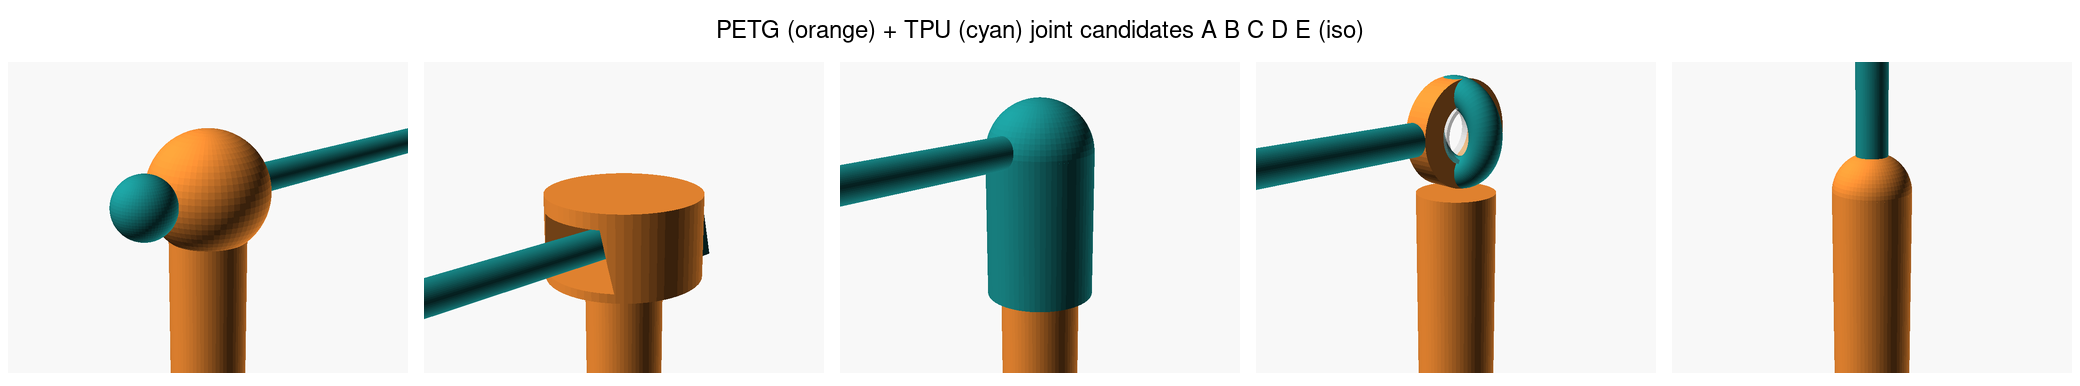
\includegraphics[width=\linewidth]{../figures/joints/all_iso_montage.png}\\[2pt]
  
\includegraphics[width=\linewidth]{../figures/joints/all_section_montage.png}
  \caption{Five candidate strut-to-cable joint geometries from the
    OpenSCAD joint study (left to right: A anchor-bulb, B dovetail,
    C TPU-sleeve overmold, D eyelet-loop, E TPU-rebar; top row
    isometric, bottom row section views). The study renders use the
    PETG (orange) + TPU (cyan) material pair under which the joint
    family was first developed; the working prototype adapts the
    selected dovetail (B) with an anchor-bulb (A) backup to the
    PLA/TPU pair of the main text, with the captive TPU core routed
    inside the PLA shell.}
  \label{fig:si-joints}
\end{figure}

% -----------------------------------------------------------------------------
\section{Support Strategy for Soft Members}
\label{si:supports}
% -----------------------------------------------------------------------------
Near-vertical TPU tendons are otherwise unsupported during printing. For the
printed campaign batches, automatic support generation was disabled and PLA
edge supports were painted manually in Bambu Studio along each tendon, with
the support-to-object XY clearance tightened from \SI{0.35}{mm} to
\SI{0.2}{mm} during tuning on the S0 reference prism
(\href{\repo/issues/98}{issue~\#98}). Support removal is the leading source of
the logged cosmetic defects (surface stringing; on two seed articles, TPU
strands pulled off bottom tendons), so defects are recorded per article in the
print key (Section~\ref{si:printkey}).

An automated alternative was developed in parallel: a tensegrity-specific
Bambu Studio recipe (support threshold angle lowered from \SI{40}{\degree} to
\SI{10}{\degree}, support material matched to the rigid extruder) combined
with manually generated narrowing pillars that ray-cast against the printable
mesh underside. The narrowing-pillar workflow is documented in
\href{\repo/pull/66}{PR~\#66}; the H2D multi-part material assignment fix is
in \href{\repo/pull/64}{PR~\#64}.

% -----------------------------------------------------------------------------
\section{As-Printed Campaign Record (Print Key)}
\label{si:printkey}
% -----------------------------------------------------------------------------
Table~\ref{tab:si-printkey} is the print key for the seed campaign: every
article's print identifier, its design, its weighed mass, and its logged
defects. The authoritative machine-readable key, together with the as-printed
slicer project (one specimen per named build plate), lives at
\href{\repo/pull/102}{PR~\#102} (\texttt{bo/t3-prism-bo-batch-print-key.csv}).
Two entries deserve care. Design 08 was printed three times; the plate label
in the archived slicer project and a contemporaneous issue comment disagree on
which article is the official one (\textit{dea4ls} versus \textit{bag26v}),
and pending confirmation the analysis uses \textit{bag26v}. The tri-print of
design 08 also supplies the only print-to-print repeatability number to date:
a mass standard deviation of \SI{0.457}{g} (three prints of a single
geometry, so not a general process repeatability estimate). Separately, one tested article
(\textit{amdjwm}) has no confirmed design mapping and is excluded from the
surrogate fit until identified.

\begin{table}[ht]
  \centering
  \caption{Print key for the seed campaign (nine Sobol designs plus the S0
    reference). Masses weighed on a \SI{0.01}{g} scale. TPU fed from a heated
    dry box near 8\% relative humidity where logged. The first five articles
    (printed before the TPU nozzle fix) used the standard \SI{0.4}{mm} TPU
    nozzle; the rest used the high-flow \SI{0.6}{mm} nozzle.}
  \label{tab:si-printkey}
  \small
  \begin{tabular}{@{}llS[table-format=2.2]l@{}}
    \toprule
    Design & Article & {Mass (g)} & Logged defects \\
    \midrule
    Spec 00 & 9hhbkp & 21.62 & none \\
    Spec 01 & 6lhxfy & 18.50 & slight strut misprint; divot on one top tendon \\
    Spec 02 & autv5r & 22.04 & minor tendon misalignment near top \\
    Spec 03 & ebdna8 & 19.61 & two strands off bottom tendons (support removal) \\
    Spec 04 & nvxsrv & 20.66 & misalignment ring after printer pause \\
    Spec 05 & 6nheas & 21.73 & two strands off bottom tendons (support-related) \\
    Spec 06 & 1zm8rv & 18.50 & stringing along diagonal tendons \\
    Spec 07 & ajhby6 & 20.53 & filament line pulled from bottom struts \\
    Spec 08 & dea4ls & 22.29 & stringing; residual PLA on tendon \\
    Spec 08 & bag26v & 21.42 & some stringing on tendon \\
    Spec 08 & ghmj4y & 22.10 & inconsistent tendon cross-section near top \\
    S0 ref. & bpx68c & 20.23 & none major \\
    \bottomrule
  \end{tabular}
\end{table}

Table~\ref{tab:si-printkey-r2} is the corresponding logged key for
the three model-recommended batches. Every batch-2 and batch-3
article printed at about 11\% dry-box relative humidity and every
batch-4 article at about 7\%. The batch-3 plate was printed twice;
the reprint articles (2dran1 to 2dran9, weighed 19.48 to
\SI{20.32}{g}, \SI{0.27}{g} heavier than the first print article for
article on average, all logged defect-free) supplied the second
test pass of the main text. The authoritative machine-readable keys,
with plate positions and the mapping evidence per row, are the
\texttt{t3-prism-bo-round1/round3/round4-print-key.csv} files
archived with the manuscript data.

\begin{table}[ht]
  \centering
  \caption{Print key for the model-recommended batches (first prints;
    the batch-3 reprint set is summarized in the text). Masses
    weighed on a \SI{0.01}{g} scale.}
  \label{tab:si-printkey-r2}
  \small
  \begin{tabular}{@{}cclS[table-format=2.2]l@{}}
    \toprule
    Batch & Trial & Article & {Mass (g)} & Logged defects \\
    \midrule
    2 & 10 & r2d2c9 & 17.91 & none \\
    2 & 11 & r2d2c4 & 19.33 & string on one top tendon; partial \\
      &    &        &       & \ \ TPU detachment \\
    2 & 12 & r2d2c2 & 17.96 & none \\
    2 & 13 & r2d2c1 & 19.38 & detached TPU string, two top \\
      &    &        &       & \ \ tendons; odd foot support \\
    2 & 14 & r2d2c6 & 19.11 & none \\
    2 & 15 & r2d2c7 & 18.51 & none \\
    2 & 16 & r2d2c3 & 18.63 & none \\
    2 & 17 & r2d2c8 & 19.98 & full-span strings, two bottom \\
      &    &        &       & \ \ tendons \\
    2 & 18 & r2d2c5 & 23.47 & none \\
    \midrule
    3 & 28 & drran5 & 19.88 & tiny bubbles, diagonal tendons \\
    3 & 29 & drran4 & 19.92 & none \\
    3 & 30 & drran9 & 19.34 & none \\
    3 & 31 & drran3 & 19.92 & tiny bubbles, diagonal tendons \\
    3 & 32 & drran7 & 20.06 & tiny bubbles, diagonal tendons \\
    3 & 33 & drran2 & 19.33 & none \\
    3 & 34 & drran6 & 19.24 & tiny bubbles, diagonal tendons \\
    3 & 35 & drran8 & 19.32 & none \\
    3 & 36 & drran1 & 19.31 & none \\
    \midrule
    4 & 37 & corny7 & 19.62 & none \\
    4 & 38 & corny2 & 20.21 & none \\
    4 & 39 & corny8 & 19.64 & none \\
    4 & 40 & corny5 & 20.58 & none \\
    4 & 41 & corny6 & 19.45 & none \\
    4 & 42 & corny1 & 20.20 & TPU mixed into one PLA strut layer \\
    4 & 43 & corny9 & 19.46 & none \\
    4 & 44 & corny4 & 20.56 & small pores, diagonal tendons \\
    4 & 45 & corny3 & 20.15 & none \\
    \bottomrule
  \end{tabular}
\end{table}

% -----------------------------------------------------------------------------
\section{Drop-Tower Protocol and Rig Characterization}
\label{si:drop}
% -----------------------------------------------------------------------------
The campaign fixture is a Lansmont Model~23 shock test system with a Test
Partner~4 data-acquisition console. The development history behind the
protocol in the main text is summarized here.

\paragraph{Protocol.} \SI{60}{in} drop height; specimen upright on the
carriage plate; first two drops of each session discarded as seating
warm-up. Session length by batch: seed sessions contribute 101
valid captures per article (103 for autv5r); the batch-2 record
lists 21 to 22 valid captures per article; batch-3 and batch-4
sessions recorded 20 drops per article. Exact per-session counts
live in the archived per-drop records, whose two generations differ
on whether the count is quoted before or after the warm-up discard.
The
shortening is justified in the main text (Section 3.3): the
statistical minimum from the pre-campaign variance study is five
stabilized drops, a truncation replay of the seed sessions preserves
the full-session transmissibility ranking at twenty drops, and the
batch-3 second pass showed the error budget is dominated by seating
and print variation rather than session length. Three slow-motion
video clips (\SI{959}{fps}) per specimen (from batch 4 filmed at
drops 1, 10, and 20 so clips pair deterministically with captures);
roughly \SI{42}{s} per drop, so about ninety minutes per seed
article and fifteen per later-batch article. Capture settings:
\SI{1.25}{MHz} sample rate, \SI{100}{ms} record, \SI{2}{ms} pre-trigger,
\SI{150}{G} trigger on the base channel, AC-coupled ICP conditioning. The
console settings were re-verified digit-for-digit against an archived
screenshot after a settings-loss event, with data continuity confirmed to
within about 1\%. Per the review instruction of 2026-09-02, the
per-session capture counts above should be re-verified by a person
against the committed per-drop records before submission.

\paragraph{Impact surface.} A blinded $3\times3$ crossover experiment over
three candidate polyurethane mat arrangements (single \SI{0.25}{in} Shore
70~OO; single \SI{0.5}{in} Shore 60~OO; stacked) selected the single
\SI{0.5}{in} Shore 60~OO sheet (\href{\repo/issues/88}{issue~\#88},
\href{\repo/pull/86}{PR~\#86}). Unlike the earlier felt stack, the mat does
not measurably compact over hundred-drop sessions. Historical note: sessions
recorded as ``5 felts'' in early protocol documents were physically four felt
sheets plus one cardboard layer.

\paragraph{Sensors and calibration.} Base input: single-axis piezoelectric
accelerometer on the carriage plate (\SI{1.059}{mV/G}, full scale
\SI{9443}{G}); top response: Dytran 3133A4 triaxial accelerometer
(X/Y/Z 0.690/0.667/\SI{0.734}{mV/G}) seated in a printed pocket at the top
vertex, mounted per ISO~5348. An earlier single-axis channel was retired
after range clipping. The two base-capable channels were cross-calibrated in
place over fifteen co-located drops: ratio $0.953 \pm 0.001$ at CFC-180
(per-drop $0.952 \pm 0.004$), stable across drop heights
(\href{\repo/pull/74}{PR~\#74}).

\paragraph{Filtering correction.} The SAE~J211/1 channel-frequency-class
filter used for all reported numbers is implemented from the standard's
published coefficients. An earlier in-house implementation passed the
two-pass (forward-backward) corner frequency to a single-pass design, which
narrows every channel class by roughly 20\% (an effective CFC-144 where
CFC-180 was intended); the discrepancy was identified during the analysis
audit of \href{\repo/issues/94}{issue~\#94} and corrected before the campaign
numbers were produced.

\paragraph{Processing pipeline.} For each capture, every channel is
calibrated and CFC-filtered independently; the top-vertex magnitude
$\lVert\mathbf{a}_{\mathrm{top}}(t)\rVert$ is formed from the three filtered
triaxial components, and the two peaks entering $t_{180}$ are searched
within a short window (approximately \SI{1.5}{ms}) of first contact, so the
peaks need not be simultaneous. The baseline is estimated from the record
tail (at healthy tower speed the mat-contact foot begins before the
\SI{2}{ms} pre-trigger window). $\Delta v$ is the integral of the baselined
base channel over the impact pulse and doubles as the rig-health gate.
Drops are discarded per the warm-up rule. Table~\ref{tab:si-processing}
collects the operational analysis parameters in one place: values known
from the protocol are stated numerically, and the remaining thresholds
are to be transcribed verbatim from the version-tagged campaign analysis
code at its archival release (a declared submission gate), rather than
paraphrased here at the risk of diverging from the code of record.

\begin{table}[ht]
  \centering
  \caption{Operational analysis parameters for the drop-tower pipeline.
    ``Code of record'' marks values to be transcribed from the
    version-tagged analysis release before submission.}
  \label{tab:si-processing}
  \small
  \begin{tabular}{@{}ll@{}}
    \toprule
    Parameter & Value \\
    \midrule
    Drop height & \SI{60}{in} (\SI{1.524}{m}) \\
    Sample rate / record / pre-trigger & \SI{1.25}{MHz} / \SI{100}{ms} / \SI{2}{ms} \\
    Trigger & \SI{150}{G} on the base channel \\
    Reporting filter class & CFC-180 (SAE J211/1), two-pass corner corrected \\
    Diagnostic filter class & CFC-1000 \\
    Peak-search window & $\approx$\SI{1.5}{ms} from first contact \\
    Baseline estimate & record tail \\
    Warm-up exclusion & first 2 drops per session \\
    Captures per session & 101 seed (103 autv5r); 21-22 batch 2; 20 batches 3-4 \\
    Rig-health check & $\Delta v$ from baselined base channel \\
    Ringdown fit gate & $r^2 \ge 0.85$ (exponential fit) \\
    Second-contact threshold and window & code of record \\
    Per-capture exclusion rules & code of record \\
    Stabilized-mean convention & code of record \\
    Filter initialization / boundary handling & code of record \\
    \bottomrule
  \end{tabular}
\end{table}

\paragraph{Rig health and repair history.} Rig health is checked
against the impact
velocity change $\Delta v$ recovered from the base channel; over an
uninterrupted 100-drop session the $\Delta v$ CV was 0.54\% with a flat
drift slope. Within a session, $\Delta v$ and the CFC-180 input
typically ease down by 1 to 4\% as the polyurethane mat warms, and
recover fully after a rest of minutes; after a mat rest or re-seat,
the first 5 to 10 drops carry the settling transient, which is why
the warm-up discard exists. The arrest velocity has visibly
stabilized as cumulative drop count grew, which is the observation
behind keeping the $\Delta v$ record even though it is no longer
listed among the paper's contributions. During commissioning, two
guide-rod locking pins failed and a
defeated pin-park safety interlock was discovered and recommissioned; the
pin-related friction produced a measurable $\Delta v$ deficit that resolved
after repair (\href{\repo/issues/92}{issue~\#92}). More than 4{,}400
instrumented drops across roughly 80 printed specimens have been
performed over about four months of commissioning, characterization,
and campaign sessions (tallied through
\href{\repo/issues/101}{issue~\#101} plus the batch records); the
campaign batches themselves contribute about 1{,}500 stabilized
captures including the batch-3 second pass.

\paragraph{Seating sensitivity, the between-seat rule, and the seat
gauge.} The batch-3 second pass (main text, Section 4.2) established
that a session can be internally stable and still misrepresent its
design: the 1.251 outlier session passed every within-session check
and did not reproduce. Two standing conventions followed. First, the
\emph{between-seat replication rule}: any single-seating value that
would drive a decision requires confirmation on an independent
re-seat. Second, an advisory \emph{seat gauge}: the broadband ratio
of CFC-1000 to CFC-180 transmissibility reads 1.00 to 1.07 in
healthy sessions, and every large same-design shift observed so far
carried a gauge of at least 1.15 in one of its seatings, so
gauge-hot sessions are treated as re-seat candidates. Both
conventions, with the session-by-session drift-watch record, live in
the drop-test datasets on
\href{\repo/pull/86}{PR~\#86}.

\paragraph{Objective provenance and adversarial review.} The objective stack
evolved through a measurability review
(\href{\repo/pull/97}{PR~\#97}): per-specimen crush energy in joules is not
recoverable from this rig (no falling-mass or displacement channel, and the
specimens stay elastic), which is why the campaign responses are the
filtered peak-acceleration ratio and a provisional mass-weighted
rebound-timing score, with quasi-static
crush metrics deferred to a load-frame campaign. A pre-registered
adversarial review of the objective choices (Edison ANALYSIS task
\texttt{3e398131}, archived in the repository) recommended
accounting for article-level rather than per-drop noise, treating
the rebound fraction as a candidate constraint pending a
restrained-versus-unrestrained validation with synchronized video,
and reserving print capacity for replicate articles. The campaign's
realized responses are recorded in the main text: the batch-3 plate
was printed and tested twice, which measured the design-level shift
distribution directly and produced the between-seat replication
rule; the rebound fraction remains a candidate constraint; and the
surrogate continues to ingest per-session standard errors, with the
replication evidence carried as an interpretation bound rather than
as an inflated noise term. The reserved-replicate recommendation now
has a planned instrument: the replicate rank-stability study of the
main-text Methods will re-print the best-, mid-, and worst-predicted
in-sample designs in nominal triplicate and test whether the
predicted ordering survives print-to-print and seating variation.

% -----------------------------------------------------------------------------
\section{Printed-Mass Model}
\label{si:mass}
% -----------------------------------------------------------------------------
The seed batch was projected onto constant \emph{solid} CAD mass
($m^{\star} = \SI{30.95}{g}$), yet the articles weigh
\SIrange{18.50}{22.29}{g}, because PLA struts print at partial infill (15\%
grid, two walls) while thin TPU cables print near solid, and the PLA-to-TPU
volume split swings widely across the design box. A two-stage calibrated
model closes this gap (\href{\repo/pull/102}{PR~\#102},
\texttt{bo/t3\_prism\_mass\_model.py}): analytic member volumes are corrected
to rendered-solid grams (one factor per material), and rendered-solid grams
are mapped to weighed grams through a wall-plus-infill term in the as-printed
strut diameter (fitted infill 23.6\%, wall \SI{1.18}{mm}, TPU factor 0.744).
The model's residual standard deviation is \SI{0.378}{g}. For context, the
three available prints of design 08 have a sample standard deviation of
\SI{0.457}{g}; three prints of one geometry are insufficient to establish a
general process repeatability limit. Inverting the model inside the
projection lets a batch hold \emph{printed} grams constant with no
slicer in the loop, and batches 3 and 4 did so at the \SI{20.23}{g}
target (the reference article's weight). Outcomes: batch mass CV
fell from 5.5\% (tested seed articles) and 8.7\% (batch 2, still
solid-mass-projected) to 1.7\% (batch 3) and 2.3\% (batch 4). The
weighings sit a few tenths of a gram below target as a per-session
flow offset ($-0.52$, $-0.25$, and \SI{-0.26}{g} for the batch-3
first print, its reprint, and batch 4), while the model's infill
terms passed their first test: regressing the print-averaged mass
residuals of the eighteen batch-3 articles on the two commanded
infills gives slopes indistinguishable from zero over the realized
13 to 34\% spread. A session-term recalibration with the accumulated
weighings is queued before the next batch's projection. Two batch-2
recommendation sets exist in the record and must not be conflated:
the batch actually sliced and sent to the printer was generated
before this correction, under the seed batch's solid-mass
projection; a subsequently regenerated set applies the
constant-printed-mass projection and seeded the batch-3 tooling.
Both are archived with the manuscript data
(\texttt{round2-as-printed-solid-mass-projection.csv},
\texttt{round3-candidate-constant-printed-mass.csv}).

% -----------------------------------------------------------------------------
\section{Metal-Analog Validation Plan}
\label{si:metal-validation}
% -----------------------------------------------------------------------------
A planned future validation campaign rebuilds a subset of the $T_3$-prism designs as
metal analogs (hollow aluminum rods for the compression members and
stainless-steel threaded cables for the tension members) using the same
$R$, $H$, $\theta$, and member-diameter parameterization as the printed
PLA/TPU specimens. To probe transfer across material systems rather than
only confirming the optimum, the selected designs deliberately span the
predicted performance range: representatives the surrogate predicts to be
worst-, mid-, and best-performing are each built in both material systems
and characterized under the identical drop protocol of
Section~\ref{si:drop}. Rank agreement between the measured PLA/TPU ranking
and the hollow-aluminum/stainless-steel ranking on the primary campaign
metric $t_{180}$ (to be reported in the main-text metal-analog table and
figure, with the provisional rebound score and, later, quasi-static SEA as
secondary rankings) would be preliminary evidence consistent with transfer
beyond the as-printed polymers; disagreement would not isolate which
material or joint difference caused the change.

\begin{figure}[ht]
  \centering
  \fbox{\parbox[c][4cm][c]{0.8\linewidth}{\centering\itshape
    Placeholder: assembled metal-analog specimens (hollow aluminum rods +
    stainless-steel threaded cables) beside their printed PLA/TPU
    equivalents for the worst/mid/best predicted tiers (photographs pending
    fabrication).}}
  \caption{Metal-analog validation specimens alongside their printed
    PLA/TPU equivalents for each predicted performance tier.}
  \label{fig:si-metal-validation}
\end{figure}

\end{document}
